\section{Results and Evaluation}
\label{sec:Auswertung}
Calculations with the resulting data are done digitally with the programming language \enquote{Python}.
Multiple packages are used, such as \enquote{Matplotlib}~\cite{matplotlib} for creating graphics, \enquote{SciPy}~\cite{scipy} for physics constants and curve-fitting and \enquote{Numpy}~\cite{numpy} for data manamgement and math support.
The uncertainty management as stated in \autoref{sec:fehlerrechnung} is done with the \enquote{Uncertainties}-package~\cite{uncertainties}.
\newline\noindent
The intensity of the $\alpha$-particles is measured by counting the events detected by the surface barrier detector.
As the measuring time interval $\increment t$ can differ between the measurements, all hit count values $C$ are normalized to \enquote{hits per second} by 
\begin{equation}
  N = \frac{C}{\increment t}\,\,\,,\,\,\,[N] = \unit{\per\second}\,.
\end{equation}
\noindent
The error for the scattering angle is determined by the resolution of the display of the rotor, which is accurate to $\increment\theta = \qty{0.1}{\degree}$.
As it is unknown how the rotor controller rounds the values inbetween, $\increment\theta = \pm\qty{0.1}{\degree}$ is taken as the absolute error for every scattering angle value. 
%
\subsection{Characteristics of the detector signal pulses}
Before the detector pulses are counted by the digital counter, the signal is amplified.
Why this is necessary can be seen when looking at the not amplified and the amplified signal pulse.
Both are shown in \autoref{fig:pulses}.
\begin{figure}
  \begin{subfigure}{0.48\textwidth}
    \centering
    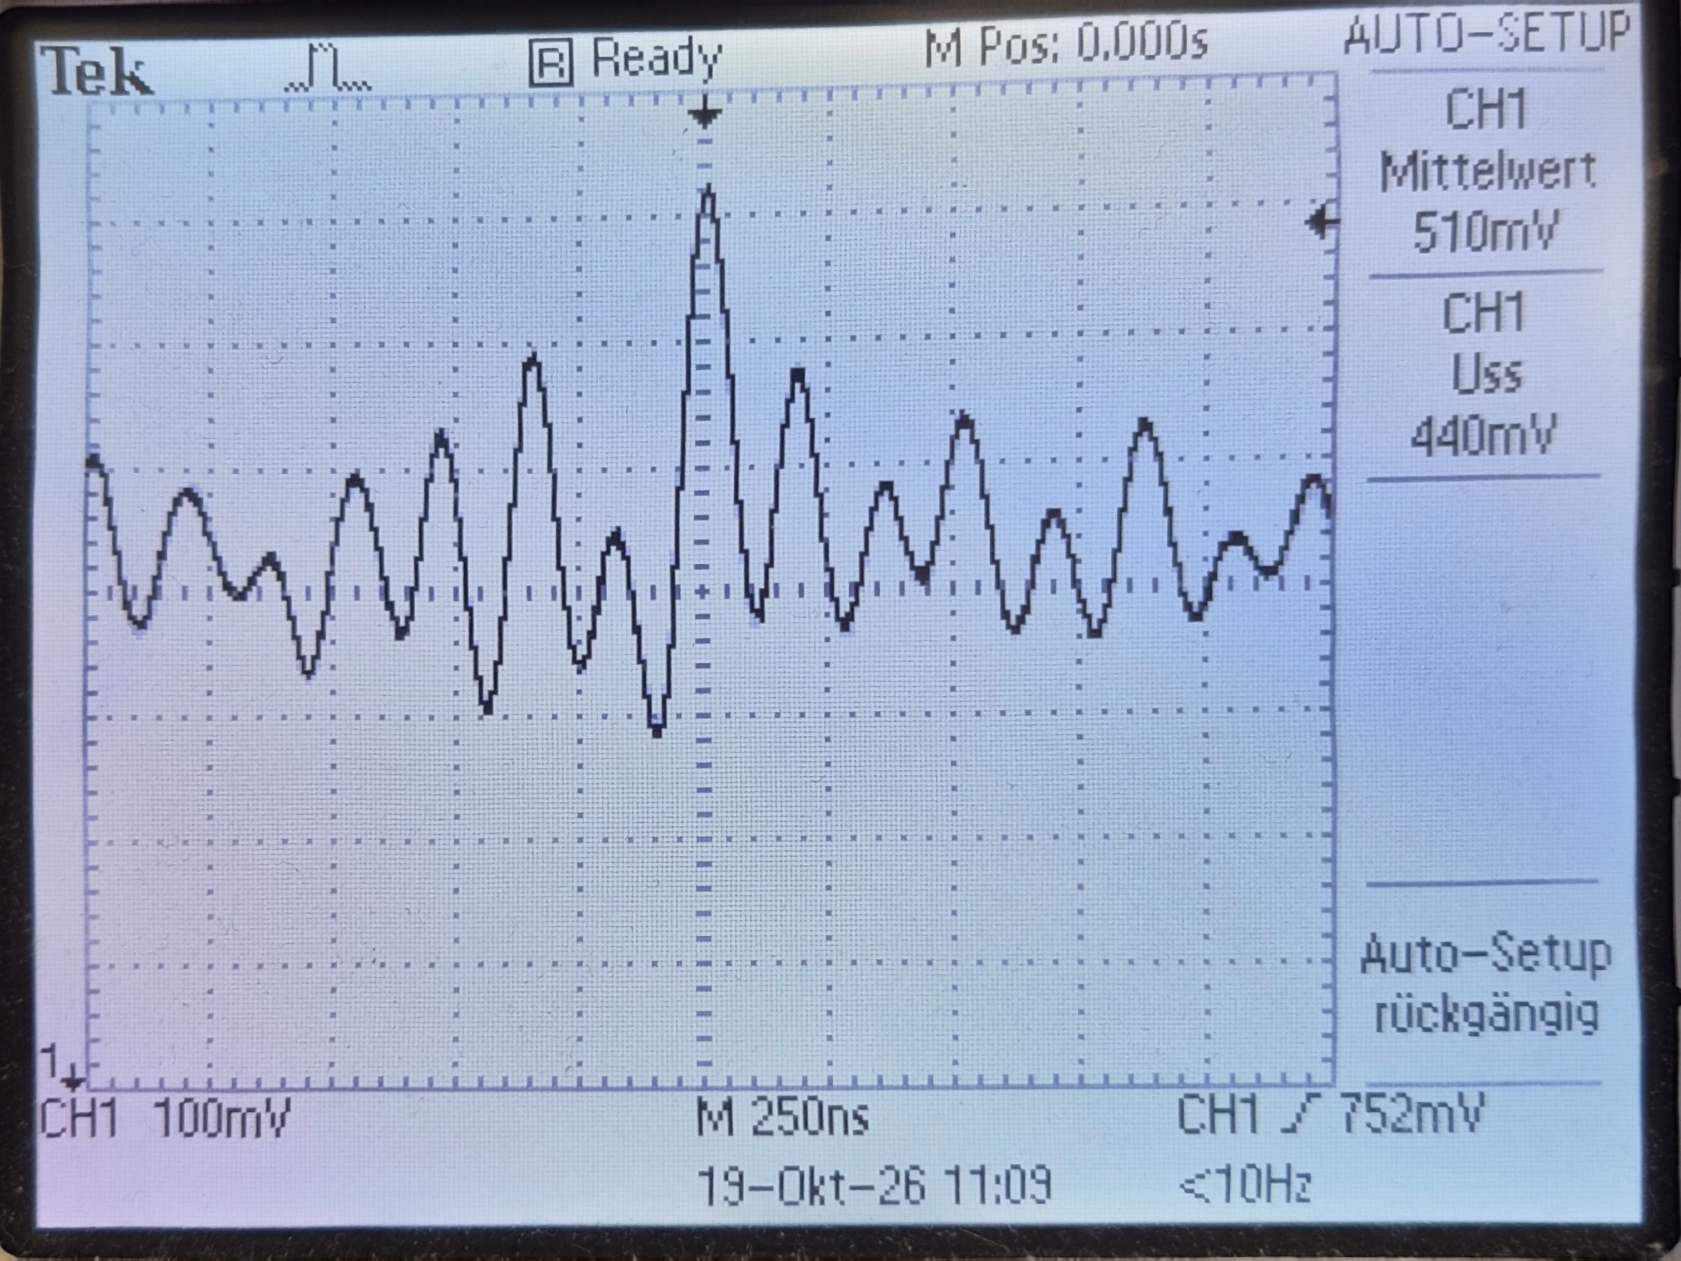
\includegraphics[height=5cm]{content/images/pre-amplified.jpg}
    \caption{Not amplified signal.}
    \label{subfig:pre}
  \end{subfigure}
  \hfill
  \begin{subfigure}{0.48\textwidth}
    \centering
    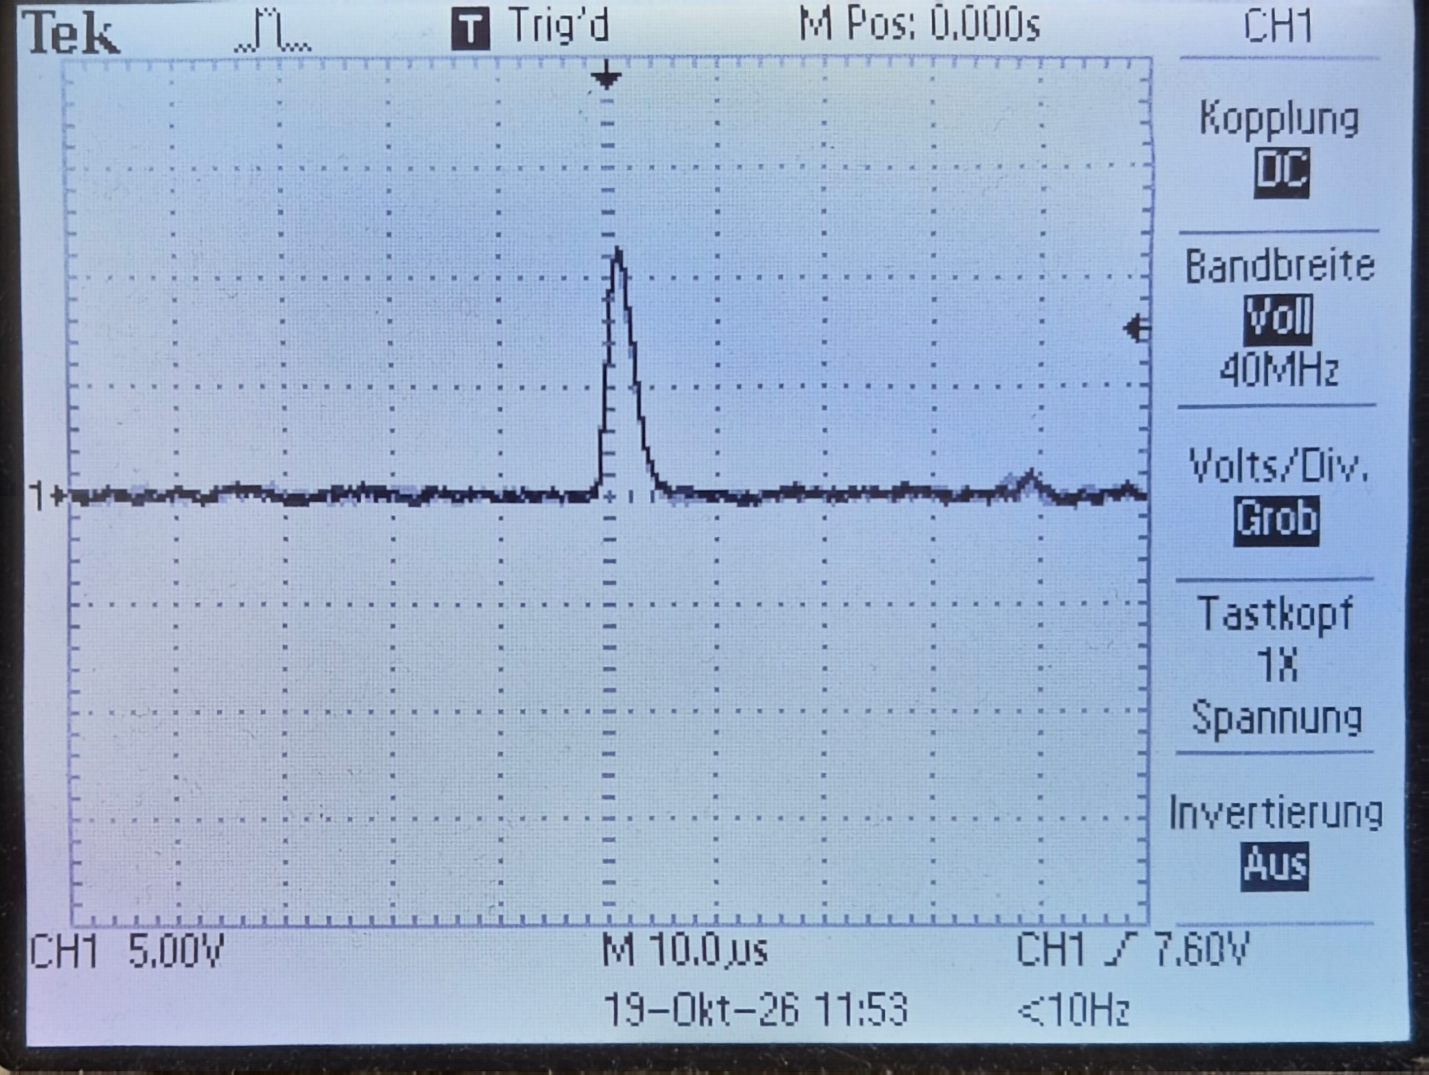
\includegraphics[height=5cm]{content/images/amplified.jpg}
    \caption{Amplified signal.}
    \label{subfig:after}
  \end{subfigure}
  \caption{Detector pulses before and after amplification, shown on a digital oscilloscope.}
  \label{fig:pulses}
\end{figure}
\FloatBarrier
\noindent
Before amplification the signal pulse is distorted by irregular signal noise, as \autoref{subfig:pre} shows.
Also, the pulse height is in the same range as the high-frequency noise, reaching $U_{\mathrm{pre}} \approx \qty{300}{\milli\volt}$. 
Therefore the signal is more likely misinterpreted by the digital counter.
In the amplified signal the detector pulse is much more distinct, with a pulse height of $U_{\mathrm{post}} \approx \qty{11}{\volt}$, as shown in \autoref{subfig:after}.
The pulse is amplified by a preset factor of $V_{\mathrm{Amp}} = \qty{16.6}{}$.
To improve the visibility of the whole pulse, the timesteps on the oscilloscope are larger for the amplified pulse than for the unamplified signal.
The noise is still visible for the amplified signal, as the baseline before and after the pulse is distorted irregulary.
%
\subsection{Beam profile measurement for calibration}
The Rutherford-experiment depends on the scattering angle, with respect to the center of the incoming beam of $\alpha$-particles.
To ensure that the beam center is aligned correctly with the surface barrier detector, the undisturbed beam profile is measured.
\autoref{fig:calibration} shows the intensity of the $\alpha$-particles depending on the scattering angle without the foil in the way and under vacuum.
The data is taken from \autoref{tab:calibration} in the appendix.
\begin{figure}
  \centering
  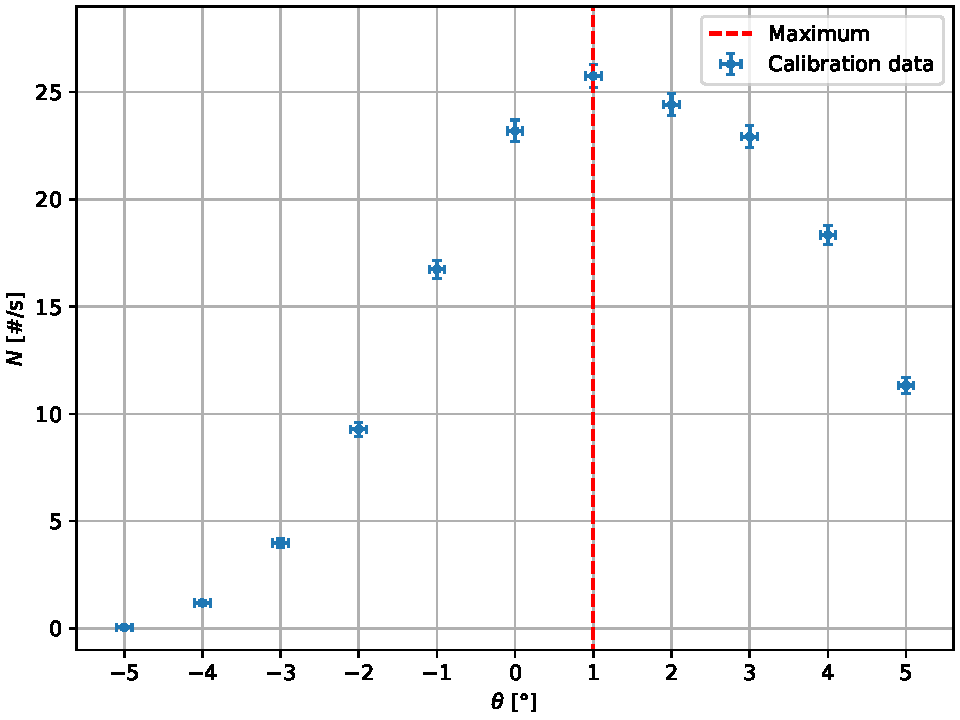
\includegraphics[width=0.7\textwidth]{content/images/calibration.pdf}
  \caption{Angular dependence of the undisturbed beam of $\alpha$-particles.}
  \label{fig:calibration}
\end{figure}
\FloatBarrier
\noindent
The beam profile shows a gaussian-like shape as expected for an undisturbed beam of particles.
Although, the center of the beam is shifted from the center defined by the angle of the rotor by $\increment\theta = \qty{1}{\degree}$.
To calibrate the rotor, the new $\qty{0}{\degree}$-point is corrected by the observed shift.
%
%
%
% \subsection{Real activity of the radiation source}
% With the maximum count rate delivered by the undisturbed beam the activity of the $\ce{^{241}Am}$ source can be calculated.
\subsection{Rutherford-scattering on gold foil}
\begin{figure}
  \centering
  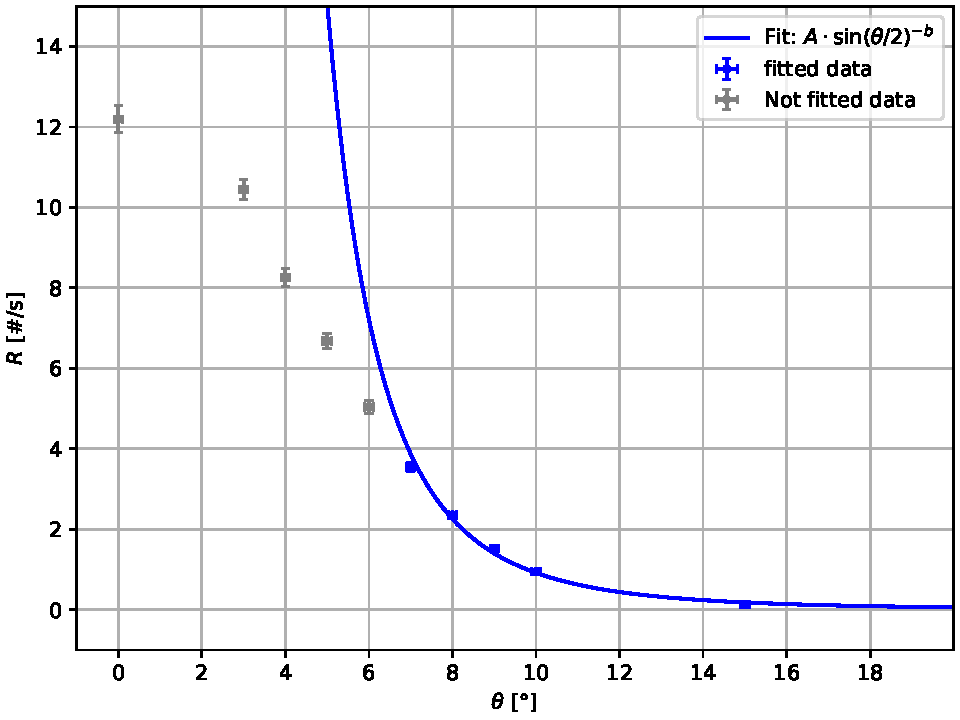
\includegraphics[width=0.7\textwidth]{content/images/Au2.pdf}
  \caption{Intensity of the $\alpha$-particles with respect to the scattering angle, scattered on $d = \qty{2}{\micro\meter}$ gold foil.}
  \label{fig:Au2}
\end{figure}
\FloatBarrier
\noindent




% \begin{figure}
%   \centering
%   \includegraphics{plot.pdf}
%   \caption{Plot.}
%   \label{fig:plot}
% \end{figure}

% \begin{table}
%   \centering
%   \caption{Eine Beispieltabelle mit Messdaten.}
%   \label{tab:tabelle}
%   \sisetup{table-format=1.1, per-mode=reciprocal}
%   \begin{tblr}{
%       colspec = {S[table-format=3.0] S[table-format=2.1] S},
%       row{1} = {guard, mode=math},
%       vline{4} = {2}{-}{text=\clap{$\pm$}},
%     }
%     \toprule
%     U \mathbin{/} \unit{\volt} & I \mathbin{/} \unit{\micro\ampere} & \SetCell[c=2]{c} N \mathbin{/} \unit{\per\second} & \\
%     \midrule
%     360 & 0.1 & 98.3 & 0.9 \\
%     400 & 0.2 & 99.8 & 1.0 \\
%     420 & 0.2 & 99.1 & 0.9 \\
%     \bottomrule
%   \end{tblr}
% \end{table}

% Siehe \autoref{fig:plot} und \autoref{tab:tabelle}!
